\documentclass[letterpaper,prl,aps,twocolumn,reprint,superscriptaddress]{revtex4-1}
\usepackage{fullpage}
\usepackage{amsmath}
\usepackage{amsfonts}
\usepackage{amssymb}
\usepackage{graphicx}
% \usepackage{slashbox}
\usepackage{color}
\usepackage{longtable}
\usepackage{array}
\usepackage{dashrule}
\usepackage[shadow,colorinlistoftodos]{todonotes}

\newcommand{\comment}[1]{{\textbf{#1}}}
\newcommand{\cotwo}{CO$_2$ }
\newcommand{\COtwo}[1]{CO$_2$ }
\newcommand{\erf}{\text{erf}}
\newcommand{\bu}{\boldsymbol{u}}
\newcommand{\bx}{\boldsymbol{x}}
\newcommand{\bz}{\hat{\boldsymbol{z}}}
\newcommand{\grad}{\boldsymbol{\nabla}}
\newcommand{\cL}{\boldsymbol{\mathcal{L}}}
\newcommand{\cA}{\boldsymbol{\mathcal{A}}}
\newcommand{\cI}{\boldsymbol{\mathcal{I}}}
\newcommand{\tc}{t_*}
\newcommand{\prt}{\boldsymbol{\xi}}
\newcommand{\nrm}{{|\cdot|}}
\newcommand{\norm}[1]{{\|#1\|}}


\newcommand{\obs}{o}
\newcommand{\inc}{i}

\begin{document}

\title{A systematic method for the linear stability of an unsteady flow}
\author{Shreyas Mandre}
\affiliation{Brown University, Providence RI 02912 USA}
\author{Anja Slim}
\affiliation{\color{red} Schlumberger-Doll Research Center, Cambridge MA 021?? USA}
\begin{abstract}
We look at solutal convection as a prototypical problem for linear stability of transient base states. 
We derive a formulation to determine the amplification of the most dangerous perturbation induced by the slowest growing norm. 
This formulation reduces to various classical and modern formulations of stability in special cases. 
We find that the threshold time for the growth of at least one perturbation in {\em every} norm (the onset of instability) agrees exactly with threshold found using frozen coefficient analysis. 
This formulation provides a rigorous justification for the frozen coefficient analysis to determine this threshold time.
\end{abstract}
\maketitle
% Background


% INTRO
A fundamental tool in fluid dynamics and beyond is linear stability analysis \cite{DrazinReid}. The idea that complexity emerges from the disruption of simple dynamics due to the growth of infinitesimally small perturbations\cite{Chandrasekhar, Drazin, etc} is found to be useful in problems like convection. The onset of linear instability therefore implies the watershed between simplicity and complexity, or at least a sufficient condition for it, such as in the case of subcritical bifurcations. 

% The idea is to look for `simple' base states, often in which some physical processes are absent, and consider whether infinitesimally small perturbations grow or decay.  If the perturbations decay, then the base state is stable and simplicity is expected for sufficiently small initial amplitudes.  Conversely, if the perturbations grow, then the base state is unstable and greater complexity will be observed.  The watershed between stability and instability is linear onset.  

% For steady base states, the concept of linear onset is clearly defined, conceptually simple and easy to calculate.  If the ensuing bifurcation is supercritical, then predictions are also in good agreement with experiments (for example in Rayleigh--Benard convection).  If the bifurcation is subcritical, then onset is observed before the linear prediction.   The extent of the discrepancy depends on the initial amplitude of the perturbations and is potentially influenced by transient, non-normal growth of otherwise stable linear modes \cite{Trefethen}.  However, the linear prediction always provides an upper bound, beyond which instability is guaranteed.  

For many applications, the relevant base state is unsteady \cite{brouillette2002richtmyer,anderson2010foam,homsy1987viscous,thorpe1968method,MORE}.  Again it is desirable to identify when a simple solution is expected an when greater complexity is likely to be observed, however the concept of onset is not clearly defined and the practice of linear stability analysis is much less clear and less well-established.  

The simplest and most obvious approach is to freeze time at a given instant and perform a standard analysis with time in the base state taken to be a parameter.  This is variably referred to as frozen-coefficient analysis or quasi-steady-state analysis.  However, this was widely criticized in the 1970s and thought to be fundamentally flawed \cite{GreshoSani71,Homsy}.  The argument is that the approach implicitly assumes that perturbations grow fast relative to the evolution of the base state, which is patently incorrect at onset.  Nevertheless, in many fields this approach is still used, albeit with the tacit understanding that it is not quite correct, presumably because it is simple in both concept and application \cite{Meiburg,BertozziBrenner}.

In other fields, there is significant research devoted to pursuing alternative calculations (for example, solutal convection in a pure fluid or in a porous medium \cite{references}).  Two popular alternatives are (1) to evolve a given set of initial conditions from $t=0$, choose a measure of size (usually an $L_2$ norm of the dependent variables) and deem onset to occur when this measure first grows or has reached a certain amplification \cite{Foster,GreshoSani,EnnisKingPaterson,more}.  In practice, the finite set is often reduced to a \emph{single} initial condition.  An alternative is (s) to choose a given shape for the perturbations for all time and calculate the amplification (with some choice of projection) \cite{Ben,Riaz,more}.  These approaches, and others, have subjective assumptions on
\begin{enumerate}
\itemsep=0cm
\item how much amplification equates to `onset'
\item the choice of time at which perturbations are introduced: usually there is continuous in time random noise and there is no \emph{a priori} reason that the relevant perturbations are introduced at $t=0$ \cite{GreshoSani}
\item the shape of perturbations
\item how to measure `size'.  For some applications, there may be a clear energy associated with the system (such as for high Reynolds number flows) that is the appropriate measure, but for many others, there is not (for example Darcy models of porous media flow or models of river braiding) and an alternative must be sought.  Even for the case of convection starting from a step-change in boundary temperature, it is debated whether the $L_2$ norm of temperature or velocity or some combination is most appropriate \cite{GreshoSani}.  Indeed, even if a clear energy is available, growth of that energy in some regions of space may be more important than in others and so may engender different weightings.
\end{enumerate}
This range of assumptions and their subjectivity can result in a wide range of predictions for onset, potentially differing by an order of magnitude or more \cite{example}.

The first subjective assumption can be made objective by defining onset of a mode as the time when its size first grows.  However, for unsteady base states, the growth of a mode does not guarantee that a macroscopic instability is observed: the mode may not be introduced at the appropriate time or may not be sufficiently amplified before the base state evolves and stabilizes.  The second and third can be made objective by assuming ignorance of the source of noise and considering all possible perturbations introduced at all possible times.  This corresponds to using generalized stability theory or non-modal analysis to find the maximum instantaneous growth rate and the amplification and specifically equating onset with zero maximum growth \cite{FarrellIoannou,SlimRama10}.  However, this still requires a choice of measure for the `size' of perturbations.

In emerging problems (Shmuel, Petia, Knobloch), people are often unsure about how to proceed.  They are aware that frozen-coefficient analysis is incorrect, but may not be aware of the applicability of generalized stability analysis, or there may not be a clear measure of size.

Thus there is a need for a clear and objective definition of onset for unsteady problems, ideally one that is conceptually and computationally simple, as well as the subsequent amplification.  We develop such definitions and explore their consequences.  We follow generalized stability analysis, but in addition to assuming ignorance of the time and type of perturbation, we also assume ignorance with respect to the measure of size.  Thus we define onset to be the {\bf earliest possible time at which in any measure of size there exists a perturbation that grows} or equivalently {\bf the earliest time at which there is no possible way of looking at the system and observing only decaying perturbations}.  In what follows, we show that this onset criterion corresponds precisely with frozen-coefficient analysis.  Thus we give a rigorous justification of frozen-coefficient analysis and the na\"ive application of steady methods to unsteady problems.  We then apply the approach to solutal convection in a porous medium as an illustrative example where non-modal stability analysis predicts a surprising result.  Amplification is defined to be the amplification of the most dangerous perturbation for the slowest growing norm.

We begin with a system of nonlinear partial differential equations representing a physical phenomenon and look for a `simple' base state.  We then consider nearby solutions by adding arbitrarily small noise and linearizing about the base state.  This yields a system of linear partial differential equations in space and time with potentially non-constant coefficients.  In practice, these partial differential equations are discretized in space using say a truncated Fourier series or a finite-difference approximation and we shall assume that they have been so \cite{FarrellIoannou}.  Thus we arrive at a non-autonomous linear system of ordinary differential equations
\begin{equation} \label{eq:GE}
\frac{\text{d}\prt}{\text{d} t} = \cL(t)\prt,
\end{equation}
where $\cL$ is the linearized operator, a potentially complex and non-normal matrix, and $\prt$ represents the discretized dependent variables, say the Fourier coefficients or point values of the dependent variables.  

The system may be formally integrated as
\begin{equation} \label{eq:PROP}
\prt (t_\obs) = \cA(t_\obs, t_\inc) \prt (t_\inc), 
\end{equation}
where $\cA (t_\obs, t_\inc)$ is the propagator for the linear system, a linear operator transforming an initial condition at time $t_\inc$ into a solution of the initial value problem at time $t_\obs$.  Substituting this form into \eqref{eq:GE} gives
\begin{equation} \label{eq:ME}
\frac{\text{d}\cA}{\text{d} t} = \cL(t)\cA,
\end{equation}
with initial condition $\cA=\cI$ at $t=t_\inc$.  The solution of this system now effectively solves the original system for all initial conditions.  For a given norm or measure of size, which we denote $\nrm$, we define the norm-dependent amplification as 
%Solving the optimization problem
\begin{align}
a_\nrm(t_\obs, t_\inc) = \max_{\prt(t_\inc)} \frac{\norm{\prt(t_\obs)}}{\norm{\prt(t_\inc)}} = \norm{\cA(t_\obs,t_\inc)}, \label{eqn:amp1} %= \max_{|\prt|=1} {| \cA(t_\obs, t_\inc) \prt|}
\end{align}
%gives 
the amplification 
%of a particular vector norm $|\cdot|$ 
induced by the most dangerous perturbation for that norm. 
Because of the time dependence of $\cL$, the amplification of the perturbation depends on both the inception time $t_\inc$ and the final time $t_\obs$, and all possible pairs $(t_\inc, t_\obs)$ must be considered. 
WE ASSUME IGNORANCE OF THE APPROPRIATE MEASURE OF SIZE?  By choosing a suitable vector norm the amplification may be made arbitrarily large, even for the most benign $\cA$ (see supplementary material?). 
To ameliorate the dependence of amplification on the choice of the vector norm, we nest the optimization to find the vector norm which results in the least amplification as
\begin{align}
a(t_\obs, t_\inc) = \min_{|\cdot|} a_\nrm (t_\obs, t_\inc). \label{eqn:amp2} % = \min_{|\cdot|} \max_{|\prt|=1} {| \cA(t_\obs, t_\inc) \prt|}
\end{align}
Defined thusly, $a$ is interpreted as the amplification of the most dangerous perturbation on the slowest growing (or least amplified) norm; 
if $a$ exists, every norm will exhibit an amplification of at least $a$ for its most dangerous perturbation.

The solution to this optimization problem is 
\begin{equation} \label{eq:RHO}
a(t_\obs,t_\inc) = \rho(\cA),
\end{equation}
where $\rho(\cA)$ is the spectral radius of $\cA$, the largest magnitude of the eigenvalues of $\cA$.  This results from two theorems of finite-dimensional linear algebra.
%The solution to this optimization is possible owing to two theorems from finite-dimensional linear algebra, and yields the optimum to be the spectral radius $a(t_\obs,t_\inc) = \rho(\cA)$ of $\cA$. 
The first 
%theorem 
states that for every vector norm $\rho(\cA) \le a(t_\obs,t_\inc)$, as can be easily verified by substituting the eigenvector corresponding to the largest magnitude eigenvalue of $\cA$ in \eqref{eqn:amp1}. 
The second 
%theorem 
states that there exists a vector norm for which the spectral radius comes arbitrarily close to $a(t_\obs,t_\inc)$ \cite{bulirsch2002introduction}; {\it i.e.} for at least one $\nrm$ and $\epsilon>0$, $\rho (\cA) + \epsilon > a(t_\obs,t_\inc)$. 
Combining the conclusions proves our claim.% that $a(t_\obs, t_\inc) = \rho(\cA)$. 
\todo[inline]{While the applicability of this conclusion is strictly valid for finite-dimensional systems, we believe that similar proofs should be possible for infinite-dimensional systems with only a few active modes ({\it e.g.} where diffusion damps out high wavenumbers, such as for \cotwo convection).}

This now allows an objective measure of amplification to be calculated via \eqref{eq:ME} and \eqref{eq:RHO}.  Instability exists when $a(t_\obs, t_\inc) > 1$.
We shall show that this definition corresponds precisely with classical analyses for steady and time-periodic base states and frozen-coefficient analysis for unsteady base states.  
%
%There are four (five?) properties of $a(t_\obs, t_\inc)$ to support the claims we make in this article. 
Here we denote the largest real part of the eigenvalues of $\cL(t)$ by $\sigma(t)$.

For steady base states, \eqref{eq:ME} can be integrated to give $\cA(t_\obs,t_\inc)= \text{e}^{\cL(t_\obs-t_\inc)}$.  Therefore the eigenvalues of $\cA$ are $\text{e}^{\sigma_j(t_\obs-t_\inc)}$, where $\sigma_j$ are the eigenvalues of $\cL$.  Hence $a(t_\obs,t_\inc)=\text{e}^{\sigma(t_\obs-t_\inc)}$ and the classical instability criterion $\sigma>0$ precisely matches our condition $a(t_\obs,t_\inc)>1$.

%{\bf Property 1:} 
%For autonomous systems, $a(t_\obs, t_\inc) = e^{\sigma (t_\obs-t_\inc)}$, where in this case $\sigma$ is independent of $t$.
%This follows from $\cA(t_\obs, t_\inc) = e^{\cL(t_\obs-t_\inc)}$, and therefore the eigenvalues $\sigma_j$, $j=1, 2, \dots$, of $\cL$ being related to the eigenvalues $e^{\sigma_j (t_\obs-t_\inc)}$ of $\cA(t_\obs,t_\inc)$.
%The classical instability criteria, $\sigma > 0$, agrees with ur criteria $a(t_\obs, t_\inc)> 1$.

%{\bf Property 2:}
For time periodic systems with period $T$, so that $\cL(t+T) = \cL(t)$, the Floquet exponents of the system ($\beta_j$) are related to the eigenvalues $e^{\beta_j T}$ of $\cA(t+T, t)$. 
Therefore, $a(t+T, t) = e^{\beta T}$, where $\beta$ is the largest real part amongst the Floquet exponents. 
For instability, the criteria according to Floquet theory is $\text{Re}(\beta) > 0$ is equivalent to $a(t+T, t) > 1$.  REFERENCE FOR FLOQUET

We now turn to onset conditions for unsteady base states.  We define onset to be the earliest time at which there is an amplified mode in every norm.  We show that this is equivalent to the earliest time at which there is an instantaneously growing mode in every norm and that this in turn is equivalent to frozen-coefficient analysis.
\todo[inline]{I think the following needs some more signposts}


{\bf Property 3:}
$a(t+\Delta t, t) = 1 + \sigma(t) \Delta t + O(\Delta t^2)$ for $\Delta t \ll 1$. 
This result follows from the expansion $\cA(t+\Delta t, t) = \cI + \cL(t) \Delta t + (\cL^2 + d\cL/dt)\Delta t^2/2 + \dots$.
The eigenvalues for $\cA(t+\Delta t, t)$ are $1 + \sigma_j \Delta t + O(\Delta t^2)$, and the spectral radius is therefore $1 + \sigma(t) \Delta t + O(\Delta t^2).$

{\bf Property 4:}
If $\sigma(t)<0$ for all $t_\inc<t<t_\obs$, then $a(t_\obs, t_\inc) < 1$.
This property follows from $\cA(t_3, t_\inc) = \cA(t_3, t_\obs) \cA(t_\obs, t_\inc)$. 
Since $\rho(AB) \le \rho(A) \rho(B)$, $a(t_3, t_\inc) \le a(t_3, t_\obs) a(t_\obs, t_\inc)$.
Therefore,
\begin{align}
 \frac{da}{dt}(t, t_\inc) &=    \lim_{\Delta t \to 0} \frac{a(t+\Delta t, t_\inc) - a(t, t_\inc)}{\Delta t} \nonumber \\
                       &\le \lim_{\Delta t \to 0} \left(\frac{a(t+\Delta t, t) - 1}{\Delta t}\right) a(t, t_\inc) \nonumber \\
                       &=   \sigma(t) a(t, t_\inc) ~ \dots ~ \text{from property 3.} \label{eqn:prop4}
\end{align}
Combined with $\sigma(t)<0$ for $t_\inc<t<t_\obs$, and $a(t_\inc, t_\inc) = 1$, we infer $a(t_\obs, t_\inc)<1$. Property 4 implies a stronger statement, $ a(t_\obs, t_\inc) \le \exp(\int_{t_\inc}^{t_\obs} \sigma(t) dt).$ The right hand side of this equation is sometimes used to quantify amplification\cite{fullana1999stability,zhang2010wavelength}, but also over-estimates the amplification. 

\todo[inline]{$\sigma(t)>0$ implies $a(t+\Delta t, t)>1$. How does one say that this means frozen coefficient works?}
For the next property, we will assume that at the earliest instance $t_0$ of interest, $\sigma(t_0)<0$, so the system is stable according to frozen coefficient analysis.
{\bf Property 5:}
The earliest time $t_\obs$ for which $a(t_\obs, t_\inc)>1$ for any $t_\inc$ is when $t_\inc=t_\obs=\tc$, where $\tc$ is the first instance at which $\sigma(t)$ becomes positive, i.e. the frozen coefficient threshold. 
We know from property 4 that $a(t_\obs, t_\inc)\le 1$, because $\sigma(t)\le 0$ for and $t$ in $t_0<t_\inc<t < t_\obs < \tc$. And from property 3 $a(\tc+\Delta t, \tc) = 1 + \sigma(\tc) + O(\Delta t^2) > 0$ for sufficiently small $\Delta t$ because $\sigma(\tc)>0$. 

Property 5 proves that the only unambiguous criteria for the onset of amplification is equivalent to the threshold from the frozen coefficient analysis.

\begin{figure}
 \centering
 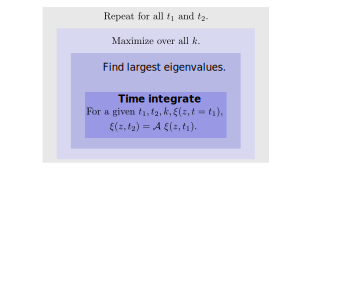
\includegraphics{./Figures/Algorithm}
 % Algorithm.pdf: 182x127 pixel, 72dpi, 6.42x4.48 cm, bb=0 0 182 127
 \caption{Schematic depiction of the nested algorithm used to find amplification $a(t_\obs, t_\inc)$ for the \cotwo convection problem. Each rectangle represents a subroutine performing the function listed in it, which is passed as a black-box to the nesting rectangle.}
 \label{fig:Algorithm}
\end{figure}

An illustrative example where generalized stability theory gives a surprising result is in solutal convection in porous media.  This problem has received significant attention recently because of its potential relevance to geological carbon dioxide storage underground in porous, brine-filled formations.  When the supercritical \COtwo{} is introduced, it is less dense than the resident brine and rises until it reaches a cap rock where it spreads laterally and forms an almost horizontal layer.  The \COtwo{} is slightly soluble in brine and dissolves into the brine cohabiting its pore space and also gradually diffuses into the underlying brine.  It has the unusual property that it makes the brine denser and so there is the potential for convective overturning.  This is of practical interest because aqueous storage is deemed to be more secure and convection greatly enhances the rate at which \COtwo{} dissolves.  Thus there is potential interest in designing injection protocols that optimize this transition.  There has been much research in the case where the two-phase layer is effectively impermeable (the brine remaining in the pore-space filled with supercritical \COtwo{} is effectively unable to flow) and a finite time for onset has been found (which could equate to hours to centuries depending on the formation properties).  However, in reality, the two-phase layer can be permeable to brine flow and where the relative permeability (the ratio of the permeability to brine in the upper, two-phase layer to the permeability in the lower, brine-only layer) is greater than about $0.5$, generalized stability analysis results suggest that onset could be instantaneous for arbitrarily thick layers.  This would strongly suggest that creating a two-phase zone that is highly permeable to brine is highly desirable.  

We readdress this problem using frozen-coefficient analysis and also calculate amplifications.  

%We now turn our attention to the case of \cotwo convection as an application of this method. 
Consider a semi-infinite layer of porous rock filled with supercritical \cotwo above a semi-infinite layer filled with brine, as shown in figure \ref{fig:Schematic}. 
We scale quantities such that the diffusivity of carbon dioxide, the Darcy mobility of the solution in the porous rock and the linear coefficient of buoyancy on \cotwo concentration is unity. 
At time $t=0$, the two layers come in contact and the \cotwo starts to dissolve and diffuse into the brine. 
The \cotwo concentration in the diffuse layer (scaled by the saturation concentration) is given by $C_0(z,t) = 1 + \erf( {z}/{2\sqrt{t}})$, where $z$ is the vertical coordinate, while the concentration in the \cotwo layer remains saturated and the fluid remains static. 
Perturbations about this state are governed by 
\begin{align}
 c_t + w C_{0,z} = \nabla^2 c \text{ and }
 \bu + \grad p + c\bz = 0
 \label{eqn:linone}
\end{align}
for $z<0$, and 
\begin{align}
 c = 0 \text{ and } \quad \bu + K (\grad p + c\bz) = 0
 \label{eqn:lintwo}
\end{align}
for $z>0$, where $c$ and $p$ are the perturbations in \cotwo concentration and pressure respectively, $\bu = (u,w)$ is the velocity, and $K$ is the ratio of mobilities in the supercritical \cotwo layer to that in the brine layer. 
We refer the reader elsewhere\cite{SlimRama10} for details. 

Given the $x$-translational invariance of (\ref{eqn:linone}-\ref{eqn:lintwo}), we decompose the $c$, $p$ and $\bu$ in Fourier modes to exploit their independent evolution with time. 
The Fourier mode with wavenumber $k$ evolves according to
\begin{align}
\begin{split}
 c_t + w C_{0,z} &= (D^2-k^2) c,  \\
(D^2-k^2)p + Dc &= 0, \quad w = -(Dp + c),
\end{split}
\end{align}
with $c=0$ and $Dp + K|k| p =0$ at $z=0$ and the symbols recycled to represent the mode amplitudes. 
The determination of amplification according to \eqref{eqn:amp2} is found using a multiply nested algorithm shown schematically in figure \ref{fig:Algorithm}. 
Each rectangle represents a subroutine for performing the function listed inside it, and is passed as a black box to the rectangle immediately outside it.
The innermost level of this algorithm is the time-integrator, which takes the initial condition $\prt(z, t_\inc)$ of wavenumber $k$ and evolves it to a given future time $t_\obs$. 
This subroutine is used by an implicitly restarted Arnoldi algorithm for iteratively finding the largest magnitude eigenvalue implemented by the ARPACK package\cite{lehoucq1998arpack}. 
The parameters $t_\inc$, $t_\obs$, and $k$ are also passed to this subroutine. 
The eigenvalue calculation routine is in turn passed as a black box to an optimization algorithm based on the golden section method to find the most dangerous wavenumber. 
This routine finds the $k$ with maximum amplification for a given $t_\inc$ and $t_\obs$. 
Finally, this optimization is repeated for a range of $t_\inc$ and $t_\obs$. 
The execution of this algorithm results in an amplification of most dangerous perturbation on the slowest growing norm for each time pair $(t_\inc, t_\obs)$. 

\begin{figure}
 \centering
 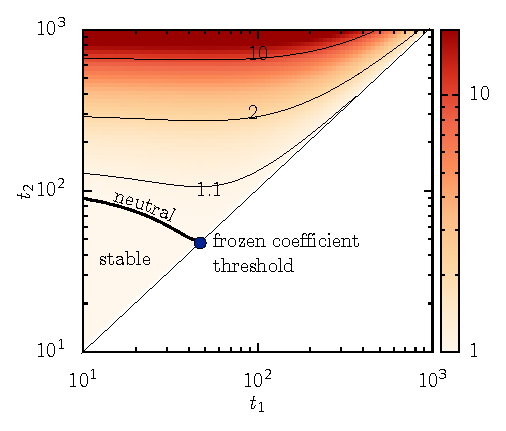
\includegraphics{./Figures/Message}
 % Message.eps: 0x0 pixel, 300dpi, 0.00x0.00 cm, bb=0 -1 227 190
 \caption{Heat map of the amplification $a(t_\obs, t_\inc)$ for the case $K=0$. Bold solid line shows the neutral curve, so that $a(t_\obs, t_\inc)=1$ below it, and $a(t_\obs,t_\inc)>1$ above. Light curves with labels show contours of constant $a(t_\obs,t_\inc)$ corresponding to the value on the label. The bold circle at $t_\obs = t_\inc = \tc$ shows the threshold according to the frozen coefficient analysis, i.e. the point for which $\sigma(\tc)=0$.}
 \label{fig:Message}
\end{figure}


\begin{figure}
 \centering
 \includegraphics{./Figures/Frozen.eps}
 % Frozen.eps: 0x0 pixel, 300dpi, 0.00x0.00 cm, bb=50 50 276 220
 \caption{a}
 \label{fig:Frozen}
\end{figure}


{\bf Results: }
The only parameter in our problem is the ratio of mobilities $K$. 
\todo[inline]{Include discussion on the role of $K$ here.}
\todo[inline]{Explain a sample amplification heat map. Interpretation of neutral curve and other contours.}
\todo[inline]{Comparison with other norms. Demonstrate that other norms always show amplification larger than the spectral radius.}
\todo[inline]{Explain properties of the threshold. The neutral curve always intersects $t_\inc = t_\obs$. The time of earliest growth (onset) is on the curve $t_\inc = t_\obs$. The neutral curve emanates perpendicular to $t_\inc=t_\obs$, when eigenvalues are real. }
Interpretation

\vspace{1cm}

Even if the amplification is greater than unity, because the perturbation is assumed to be infinitesimal in magnitude, it is not possible to determine based on the linear amplification analysis alone whether the growing perturbation will visibly alter the system. 
Knowledge of the statistical distribution of spectrum of initial perturbations or the external influences feeding the perturbation is needed to make such a prediction in this framework. 
This difference compared to the autonomous case had been identified by previous researchers on the topic.

(modal ansatz cannot be made)

\bibliography{timevariant,others}
% \bibliographystyle{}

\newpage
\section*{Supplementary material}
As an illustration, consider the case where the propagator is represented by a $2\times 2$ diagonal matrix,
\begin{align}
 \begin{bmatrix} x_1 \\ x_2 \end{bmatrix}
 \to
K \begin{bmatrix} 1 & 0 \\ 0 & 5 \end{bmatrix}
 \begin{bmatrix} x_1 \\ x_2 \end{bmatrix}.
 \label{eqn:exoperator}
\end{align}
Clearly, if the 2-norm $|x| = \sqrt{x_1^2 +x_2^2}$ is used, the amplification induced by this matrix is $5K$, corresponding to the stretching in the $x_2$ direction. Choosing the scaling factor $K$ allows us to arbitrarily change this norm, and choosing $K<1/5$ causes the operator to be diminishing, rather than amplifying. Now consider the coordinate transformation
\begin{align}
 \begin{bmatrix} u_1 \\ u_2 \end{bmatrix}
 =
 \begin{bmatrix} (1+\epsilon) & -(1-\epsilon) \\ (1-\epsilon) & -(1+\epsilon) \end{bmatrix}
 \begin{bmatrix} x_1 \\ x_2 \end{bmatrix}.
 \label{eqn:transform}
\end{align}
In the $(u_1, u_2)$ coordinates, the same abstract operator in \eqref{eqn:exoperator} is represented by the matrix
\begin{align}
 \begin{bmatrix} u_1 \\ u_2 \end{bmatrix}
 \to \frac{K}{\epsilon}
 \begin{bmatrix} -1+3\epsilon-\epsilon^2 & 1-\epsilon^2 \\ -1+\epsilon^2 & 1+3\epsilon+\epsilon^2 \end{bmatrix}
 \begin{bmatrix} u_1 \\ u_2 \end{bmatrix}
\end{align}
Using $|u| = \sqrt{u_1^2 + u_2^2}$, the norm of this matrix diverges as $2K/\epsilon$ as $\epsilon$ approaches zero. Such a divergence is closely linked to the choice of the basis used to represent the vector space (as $\epsilon\to 0$, the eigenvectors are almost but not exactly parallel to each other in this representation, whereas the eigenvectors of the matrix in the first representation were orthogonal). Irrespective of $K$, choosing $\epsilon < 2K$ causes this norm to be greater than unity. 

The equivalence between the choice of the basis for the vector space and the choice of the vector norm used in the definition of the operator norm, is also clearly visible in this illustration. The same result could be obtained by transforming the norm instead of the coordinates. If $|x| = \sqrt{u_1(x_1,x_2)^2 + u_2(x_1,x_2)^2}$, where $u_{1,2}(x_1, x_2)$ are given by \eqref{eqn:transform}. The growth induced on this norm will approach $2K/\epsilon$. Similarly, using the vector norm $|u| = \sqrt{x_1^2(u_1,u_2)+x_2^2(u_1,u_2)}$ is equivalent to transforming back to the $(x_1, x_2)$ coordinates and using the $L_2$-norm in $(x_1, x_2)$, and thus will result in the operator norm equal to $5K$. This behavior of the amplification induced by the operator extends to all other vector norms, although we have demonstrated it using quadratic norms.

This illustration highlights the following conundrum a theorist faces when using operator norms to study the amplification caused by a linear map. Suppose a large operator norm is observed while performing a stability analysis of a dynamical system, how much of this operator norm is an inherent property of the underlying abstract linear operator and how much is due to the choice of a basis used to represent the dynamical system? Note that, as illustrated in the above example, the spurious artifact from a bad choice of the basis is especially exaggerated when the eigenvectors are nearly parallel, as is the case for many non-normal representations of linear operators.

\end{document}
